\section{Frontend} \label{sec:Frontend}
Für die Realisierung des Frontends sollte aus den in \autoref{chap:Entwurf} genannten Gründen auf ein bestehendes Framework zurückgegriffen werden. In der Betrachtung werden die drei beliebtesten JavaScript Frameworks, laut einer Stackoverflow (Frage- und Antwortseite für Programmierende) Umfrage, diskutiert. Die Umfrage, bei der circa 65.000 Menschen teilgenommen haben, wurde im Februar 2020 durchgeführt. \cite{stackexchangeStackOverflowDeveloper2020}

\begin{center}
	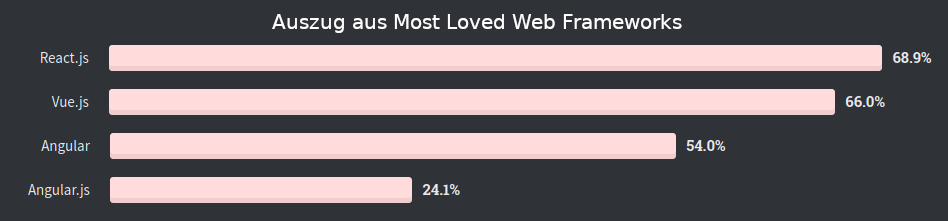
\includegraphics[width=\linewidth, keepaspectratio]{technologie/so-loved-fw}
	\captionof{figure}{Weiterverwendung des benutzten Webframeworks (Screenshot) \cite{stackexchangeStackOverflowDeveloper2020}}
	\label{fig:frontend-so-loved}
\end{center}

\begin{center}
	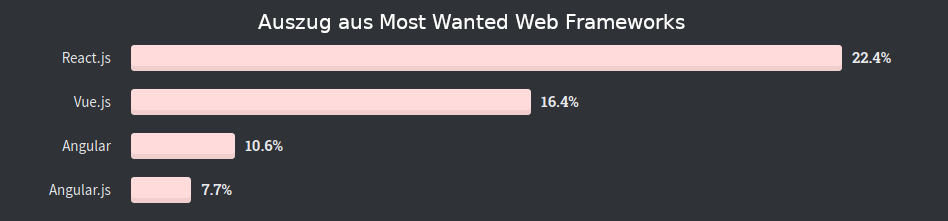
\includegraphics[width=\linewidth, keepaspectratio]{technologie/so-wanted-fw}
	\captionof{figure}{Interesse an einem neuen Webframework (Screenshot) \cite{stackexchangeStackOverflowDeveloper2020}}
	\label{fig:frontend-so-wanted}
\end{center}

In der \autoref{fig:frontend-so-loved} ist zu sehen, wie viele Prozent der Entwickelnden, welche bereits mit der Technologie arbeiten, ein Interesse bekundet haben, diese für weitere Projekte zu nutzen. React.js führt diese Liste mit 69 \% an. Darauf folgt Vue.js dicht mit 66 \%. Bei Angular sieht es etwas anders aus, hier bekunden nur 54 \% ein Interesse. Im Gegensatz dazu wollen $\sim$25 \% der Befragten den Vorgänger Angular.js weiter nutzen.

Die \autoref{fig:frontend-so-wanted} zeigt in Prozent, wie viele der Entwickelnden ein Interesse an der Technologie haben, bisher aber noch nicht mit dieser gearbeitet haben. Auch hier ist React.js mit $\sim$22 \% führend. Etwas abgeschlagen mit $\sim$16 \% folgt Vue.js. Dahinter reihen sich Angular mit $\sim$11 \% und Angular.js mit 8 \% ein.

\begin{center}
	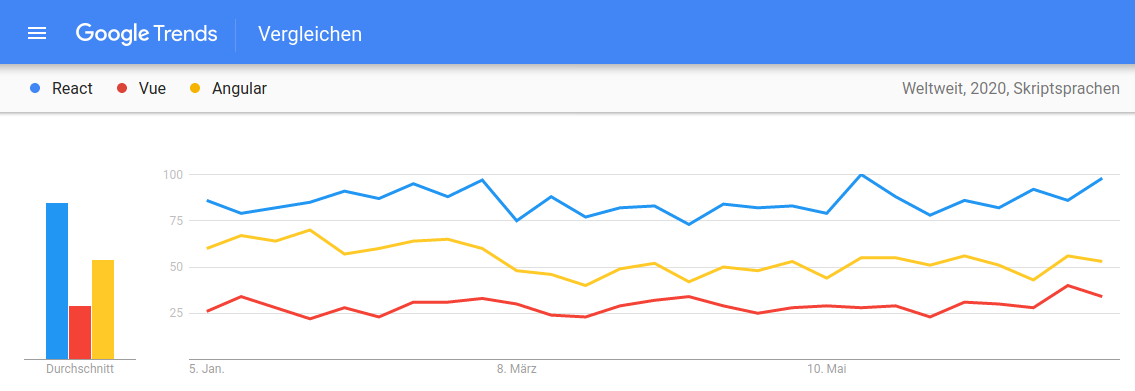
\includegraphics[width=\linewidth, keepaspectratio]{technologie/google-trends}
	\captionof{figure}{Google Trends (Screenshot) \cite{googleGoogleTrends2020}}
	\label{fig:frontend-google-trends}
\end{center}

\begin{center}
	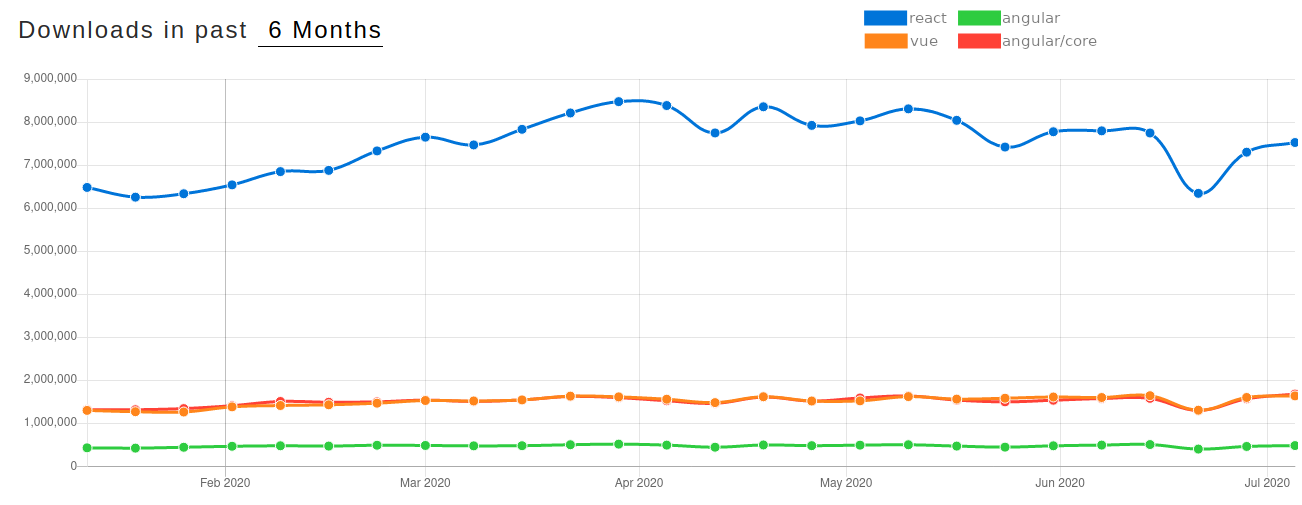
\includegraphics[width=\linewidth, keepaspectratio]{technologie/npm-trends}
	\captionof{figure}{NPM Trends (Screenshot) \cite{potterReactVsVue2020}}
	\label{fig:frontend-npm-trends}
\end{center}

Die Google Trends in \autoref{fig:frontend-google-trends} zeigen das aus Stichproben normalisierte Interesse an einem Begriff vom Januar 2020 bis Anfang Juli 2020. Das Interesse wird von Google stichpunktartig anhand von Google Suchanfragen bestimmt. \cite{googleHaufigGestellteFragen2020}

In der \autoref{fig:frontend-npm-trends} werden die wöchentlichen Downloads pro Framework grafisch dargestellt. In dieser ist erkennbar, dass Vue.js und Angular ungefähr gleich oft heruntergeladen werden. Generell ist eine Stagnation der Frameworks erkennbar, einzig bei React.js schwanken die Downloadzahlen zwischen 6,5 und 8,5 Millionen. Derzeitig scheinen sich die Downloads bei ungefähr 7 Millionen pro Woche eingependelt zu haben.

Durch die \autoref{fig:frontend-so-loved}, \autoref{fig:frontend-google-trends} und \autoref{fig:frontend-npm-trends} lässt sich schlussfolgern, dass React.js derzeitig das beliebteste und auch verbreiteteste Framework ist. Das unbeliebteste Framework der Auswahl scheint Angular.js zu sein. Anhand der Grafiken fällt eine klare Positionierung von Vue.js und Angular zwischen React und Angular.js schwer.

Im Folgenden sollen die Frameworks genauer betrachtet werden, um eine Nutzung unter anderem anhand des Funktionsumfangs, der Mächtigkeit sowie der Komplexität zu beurteilen.

\subsection{Angular}
AngularJS wurde von einem Google Mitarbeiter (Misko Hevery) als Seitenprojekt gestartet. Das Nebenprojekt wollte er nutzen, um interne Webanwendungen einfacher zu entwickeln. Nachdem einige interne Anwendungen mit diesem Projekt erstellt worden sind, wurde AngularJS im Jahr 2010 als Open-Source-Projekt veröffentlicht. Es fand sowohl in Unternehmensprojekten als auch in Projekten der Open-Source Community Anwendung. \cite{gaviganHistoryAngular2018}

Einige Jahr nach der Veröffentlichung, begann sich die Landschaft der Webentwicklung durch Weiterentwicklungen und neue Standards in JavaScript zu verändern. Neben dieser Veränderung ist das Team an die Grenzen gestoßen, welches die Verbesserung des Frameworks anging. Dieses führte dazu, dass AngularJS über die Zeit an Modernität verlor. \cite{gaviganHistoryAngular2018}

AngularJS war beim Entwurf nie für Mobile oder Unternehmensanwendungen gedacht.
So entschied sich das Team bei Google mit der Entwicklung der Version 2 einen Neuanfang zu wagen und Angular 2 für solche Anwendungsfelder zu entwerfen. \cite{gaviganHistoryAngular2018}

Um Verwirrungen zu vermeiden, wurde das bis dahin bekannte Angular in AngularJS umbenannt und die neue Version Angular 2 genannt. Des Weiteren folgt die Versionierung von Angular seit Version 2 dem Semantic Versioning Prinzip bei dem die Versionsnummer in \textquote[\cite{preston-wernerSemanticVersioning}]{MAJOR.MINOR.PATCH} untergliedert wird. \cite{gaviganHistoryAngular2018} 

In der Anfangsphase von Angular 2 war es umständlich ein neues Projekt anzulegen, die Build-Größen waren vergleichsweise groß. So erarbeitete sich Angular den Ruf sperrig zu sein.
Neben diesem wurde in Version 2 die Sprache von JavaScript zu TypeScript (Obermenge von JavaScript) umgestellt, welches unter anderem eine andere Syntax und neue Konzepte zur Folge hatte. \cite{gaviganHistoryAngular2018}

Am 24.06.2020 erschien Angular2 in der Version 10.0.0 \cite{googleAngularAngularVersioning2020} und zählt wie bereits vorher dargestellt zu den beliebtesten Frontend-Frameworks.

Im Folgenden wird nur das aktuell beworbene Angular2 dargestellt und Angular genannt.

Bei der Entwicklung von Angular wurde auf Konsistenz, Produktivität, Wartbarkeit, Modularität und frühzeitige Fehlererkennung gesetzt.

Angular 2 basiert auf Komponenten und Diensten, welche alle identische Strukturen besitzen. Auch gibt Angular vor, wie wiederverwendbarer Code angelegt wird, sodass hierfür keine Code Styles notwendig sind. Des Weiteren erhält die Angular Dokumentation einen Style-Guide. So müssen die Unternehmen keinen eigenen Style-Guide erstellen, was eine Zeitersparnis darstellt. Durch diesen konsistenten Aufbau wird auch eine bessere Wartbarkeit gewährleistet. \cite{wahlinWesentlichenVorteileAngular2017}

Durch die Konsistenz, die gegebenen Style-Guides und den wiederverwendbaren Code steigt die Produktivität, da die Entwickelnden eingeschränkter sind und nicht überlegen und bewerten müssen, ob das aktuell angewandte Vorgehen richtig ist.  \cite{wahlinWesentlichenVorteileAngular2017}

Die Wartbarkeit der geschrieben Anwendung profitiert von der Konsistenz und den Style Guides, da so jeder der involviert ist, den Code leichter nachvollziehen und verändern kann. Derzeitig ist durch das große Interesse der Community sowie der internen Nutzung bei Google, die Wartbarkeit des Frameworks gesichert. \cite{wahlinWesentlichenVorteileAngular2017}

Bei Angular wird der Code in einzelne Module organisiert. Durch die Nutzung des modularen Systems können diverse Teams derselben Anwendung arbeiten, ohne sich gegenseitig zu behindern. \cite{wahlinWesentlichenVorteileAngular2017}

Die frühzeitige Fehlererkennung wird durch die Nutzung von TypeScript ermöglicht. TypeScript bietet im Gegensatz zu JavaScript Unterstützung für Typisierung. Die Nutzung der Typen ist in TypeScript nicht vorgeschrieben, aber zur Fehlererkennung empfohlen.
Des Weiteren ermöglicht das Angular-CLI eine einfache Methode um Unittests und End-zu-End-Tests durchzuführen, so können Fehler entdeckt und behoben werden. \cite{wahlinWesentlichenVorteileAngular2017}

Diese Vorgaben führen zwar zu einer besseren Wartbarkeit und einer konsistenten Anwendung, schränken aber zeitgleich Entwickler ein. Um eine konsistente Anwendung zu erhalten, ist das Gerüst unflexibel.

Da Angular in Unternehmensanwendungen verwendet werden soll, ist es komplex und benötigt so eine gewisse Einarbeitungszeit. Diese steile Lernkurve muss von neuen Programmierenden bewältigt werden. \cite{ventzkemediaAngularVsReact2018}

\subsection{React}
Im Jahr 2010 startete React als Port von XHP (PHP-Erweiterung, welche XSS Angriffe vorbeugen sollte) bei Facebook. Da XHP Probleme mit dynamischen Webanwendungen nicht löste, bat ein Facebook Software-Engineer um Zeit, damit er XHP unter zur Hilfenahme von JavaScript in den Browser bringen könne. \cite{dawsonJavaScriptHistoryHow2014}

Anfänglich wurde React noch unter \textquote{BSD  + patents} lizenziert. Diese Lizenz gewährte eine Nutzungslizenz und eine Patentlizenz, solange von einer Klage gegen Facebook bei möglichen Patentverletzungen abgesehen wird. Am 25 September 2017 wurde die Lizenz nach Kritik zu \textquote{MIT} gewechselt. \cite{kripalaniIfYouRe2017} \cite{larsonFacebookJustChanged2017} Die MIT-Lizenz ist eine sehr wenig restriktive Lizenz und gibt die Erlaubnis zur Veränderung, Modifikation und Nutzung ohne Kosten. Des Weiteren beinhaltet diese kein Copyleft. Bei einem Copyleft muss das entwickelte Produkt (hier die Software), welches die Software mit Copyleft nutzt, unter derselben Lizenz veröffentlicht werden. \cite{wehnerSoftwareUnterMIT2020}

React besteht aus Komponenten und nutzt eine Syntaxerweiterung von JavaScript namens JSX, um JavaScript und HTML zusammenzuführen. Die JSX-Dateien müssen vor der Auslieferung  an den Client in JavaScript transformiert werden. Reacts Komponenten sollten möglichst klein sein und nur eine Aufgabe erledigen. Diese führt zu einer besseren Test- und Wartbarkeit sowie einem besseren Verständnis der Anwendung. \cite{bezJavaScriptEinfuehrungReact2015}

Auch nutzt React für seine React Views einen sogenannten Virtual DOM (Document Object Model). Die Nutzung der React Views ermöglichen es, die Anwendungen auf dem ausliefernden Server zu rendern. Neben diesem können Unterschiede zwischen DOM und vDOM erkannt werden. Dadurch muss nicht mehr die gesamte Seite sondern nur die veränderte Komponente neu gerendert werden. Dieses resultiert in einer besseren Performance. \cite{bezJavaScriptEinfuehrungReact2015}

Um Beispielsweise eine SPA in React zu entwickeln muss auf Drittanbieter Erweiterungen zurückgegriffen werden oder die entsprechenden Funktionen müssen selber programmiert werden, da diese nicht in React enthalten sind. Dies stellt entweder Zeitaufwand oder Abhängigkeiten von weiteren Entwicklern dar.

\subsection{Vue}
Vue.js wurde durch einen damaligen Mitarbeiter von Google (Evan You) entworfen und entwickelt, nachdem er viel mit Angular gearbeitete hatte. Er wollte nur einen ganz kleinen Teil aus Angular nutzen. So begann er zunächst nur für sich, veröffentlichte aber im Februar 2014 die Version 1.0.0 auf GitHub. \cite{teufelVueJsTutorial2018}

Das Projekt gewann Beliebtheit auf GitHub und die Community beteiligte sich. Die ersten Plugins wurden geschaffen und es bildete sich ein Core Team.

Vue liefert im Gegensatz zu den anderen vorgestellten Frontend-Frameworks nur das Data Binding und die Möglichkeit Komponenten zu programmieren im Kern mit. Zusätzlich benötigte Funktionen können bei Bedarf als Module geladen werden. Dies macht Vue zu einem spezialisierten aber auch universell nutzbaren Framework. Es ist nicht so universell nutzbar wie Angular aber auch nicht so spezialisiert wie React. \cite{teufelVueJsTutorial2018}

Die Dokumentation von Vue ist leicht verständlich und die Community hilft schnell bei Fragen. Anwendungen in Vue sind in eine hierarchische Struktur von kleinen Komponenten untergliedert. Dies soll ermöglichen, dass die Komponenten und so das gesamte System besser zu verstehen sind. Redundanz ist dort zulässig, wo diese benötigt wird.
Komponenten erhalten neben dem reinen HTML auch CSS und JavaScript und sollen atomar sein. Das heißt, dass diese alleine und ohne Bindungen zu einer Komponente in einer logisch gesehen höher liegenden Ebenen nutzbar sind. Durch diesen Ansatz ist die Software übersichtlicher, was zu einer besseren Test- und Wartbarkeit führt. \cite{teufelVueJsTutorial2018a}

Damit diese Trennung nicht nur in der Software, sondern auch auf der Dateiebene passiert, nutzt Vue hierfür die sogenannten Single File Components. Diese Dateien enden mit der Dateiendung \textit{.vue} und sind erst nach einer \textquote{Kompilierung} nutzbar. Eine Single File Component trennt HTML, CSS und JavaScript auf, sodass dieses übersichtlich betrachtetet werden kann. \cite{teufelVueJsTutorial2018a}

Ein Nachteil von Vue ist, dass es von keiner großen Firma entwickelt wird, welche die Entwicklung vorantreibt und die Verbreitung erhöht. Des Weiteren werden Angular und React intern selber genutzt, sodass das Framework eine langfristige Nutzung hat. Aber seit circa 2016 nutzen immer mehr Unternehmen Vue. Hier sind beispielsweise GitLab (2016, \cite{schatzWhyWeChose2016}), Laravel und Nintendo zu nennen. \cite{techuzTopWebsitesBuilt2018}

\subsection{Wahl des Frontend-Frameworks}

Für das Frontend sollte entweder Vue oder React genutzt werden, da diese einsteigerfreundlicher sind. Angular wird auf Grund der Komplexität und des Umfangs des zu schreibenden Frontends nicht in Betracht gezogen. Sowohl für Vue als auch für React sprechen ausreichend Gründe. 

Vue ist schlanker und etwas leichter zu erlernen als React, da hier nur Kenntnisse in JavaScript, CSS und HTML benötigt werden. Bei React werden noch zusätzliche Kenntnisse in JSX benötigt.

Für React spricht die Verbreitung und die damit größere Community, welche bei Problemen konsultiert werden kann. Auch ist es wahrscheinlicher, dass Problemstellungen bereits auf Frage-Antwort Plattformen wie StackOverflow behandelt worden sind. 

Schlussfolgernd sollte für das Frontend React genutzt werden, da hier eine größere Community bei Fragen zur Verfügung steht.
